\documentclass[a4paper, 12pt]{article}

% Поддержка русского языка
\usepackage[english, russian]{babel}
\usepackage[T2A]{fontenc}
\usepackage[utf8]{inputenc}
\usepackage{indentfirst}
\usepackage{hyperref}
\usepackage{graphicx}
\usepackage{wrapfig}
\usepackage{sidecap}

\usepackage{amsmath, amsfonts, amssymb, amsthm, mathtools}

%% Оформление страницы
\usepackage{extsizes}     % Возможность сделать 14-й шрифт
\usepackage{geometry}     % Простой способ задавать поля
\usepackage{setspace}     % Интерлиньяж
\usepackage{enumitem}     % Настройка окружений itemize и enumerate
\setlist{leftmargin=25pt} % Отступы в itemize и enumerate

\geometry{top=25mm}    % Поля сверху страницы
\geometry{bottom=30mm} % Поля снизу страницы
\geometry{left=20mm}   % Поля слева страницы
\geometry{right=20mm}  % Поля справа страницы

\setlength\parindent{15pt}        % Устанавливает длину красной строки 15pt
\linespread{1.3}                  % Коэффициент межстрочного интервала
%\setlength{\parskip}{0.5em}      % Вертикальный интервал между абзацами
%\setcounter{secnumdepth}{0}      % Отключение нумерации разделов
%\setcounter{section}{-1}         % Нумерация секций с нуля
\usepackage{multicol}			  % Для текста в нескольких колонках
\usepackage{soulutf8}             % Модификаторы начертания

% Титульный лист
\newcommand{\ProjectName}{Луна-9}
\newcommand{\FullProjectName}{Луна-9}

\usepackage{titleps}
\newpagestyle{main}{
	\setheadrule{0.1pt}
	\sethead{Проект по ВвАРКТ <<\ProjectName>>}{}{}
	\setfootrule{0.1pt}
	\setfoot{ПМИ МАИ, 2022}{}{\thepage}
}
\pagestyle{main}
\newcommand{\tus}{\textunderscore}

\begin{document}
\begin{center}
	\huge{Проект по ВвАРКТ <<Луна-9>>} \\
	\large{(Первое в истории мягкое прилунение)} \\
	\Large{Project Research Document}\\
	\large{\textbf{Медведев Е.А}, Медведев Н.А, Кабанов А.А, Новиков Н.С, Мунтяну А.В} \\
	\large{(команда <<Луна-9>> / М8О-101Б-22)}
	\rule{\textwidth}{0.1pt}
\end{center}

\section*{Введение}
\noindent Любой ребенок, смотря в звездное небо, невольно устремляет свой взгляд к Луне. Это небесное тело эффектно выделяется на фоне остальных огоньков в небе. Но наука тоже не остается в стороне и активно изучает все небесные тела, которые только возможно. Так, ученые уже знают практически все про естественный спутник Земли, однако так было не всегда. Как же человечество смогло собрать столько информации о теле, находящемся на огромном расстоянии от нашей планеты? Наша команда, заинтересовалась данным вопросом,  мы выбрали именно эту знаковую миссию, ведь <<Луна-9>> совершила первую мягкую посадку на Луну и смогла передать человечеству первые снимки с ее поверхности. 
\paragraph{Цель} Провести симуляцию миссии <<Луна-9>> в KSP, научиться работе с библиотекой kRPC, написать программу, получающие данные о полете во время симуляции в KSP, сравнить результаты работы программы с результатами, полученными с помощью математиечской и физической моделей.
\subsubsection*{Задачи}
\begin{enumerate}
	\item изучить доступную информацию о полете <<Луна-9>>;
	\item проанализировать ее;
	\item произвести расчеты и создать математическую и физическую модели;
	\item осуществить сборку аналогичной ракеты в KSP;
	\item запрограммировать функции подсчета основных параметров ракеты и ее полета;
	\item реализовать миссию в KSP:
	\begin{enumerate}
		\item вывести ракету на орбиту Земли;
		\item выход с орбиты Земли;
		\item преодолеть расстояние между Землей и Луной;
		\item выход на орбиту Луны;
		\item мягкая посадить на Луну;
		\item развернуть АЛС;
		\item сделать несколько снимков поверхности Луны;
	\end{enumerate}
	\item сравнить показания собственных функций с действительными.
\end{enumerate}
\subsection*{Команда}
\begin{tabular}{|c|c|}
	\hline 
	Кабанов А.А	& KSP-программист \\
	\hline
	Медведев Н.А & Программист \\
	\hline
	Медведев Е.А & Физик, тимлид \\ 
	\hline
	Новиков Н.С & Тестировщик, программист \\ 
	\hline
	Мунтяну А.В	& Математик \\
	\hline
\end{tabular}


\section{Описание миссии}
\subsection{Описание миссии и исторические справки}
\begin{wrapfigure}{r}{0.3\textwidth} %this figure will be at the right
	\centering
	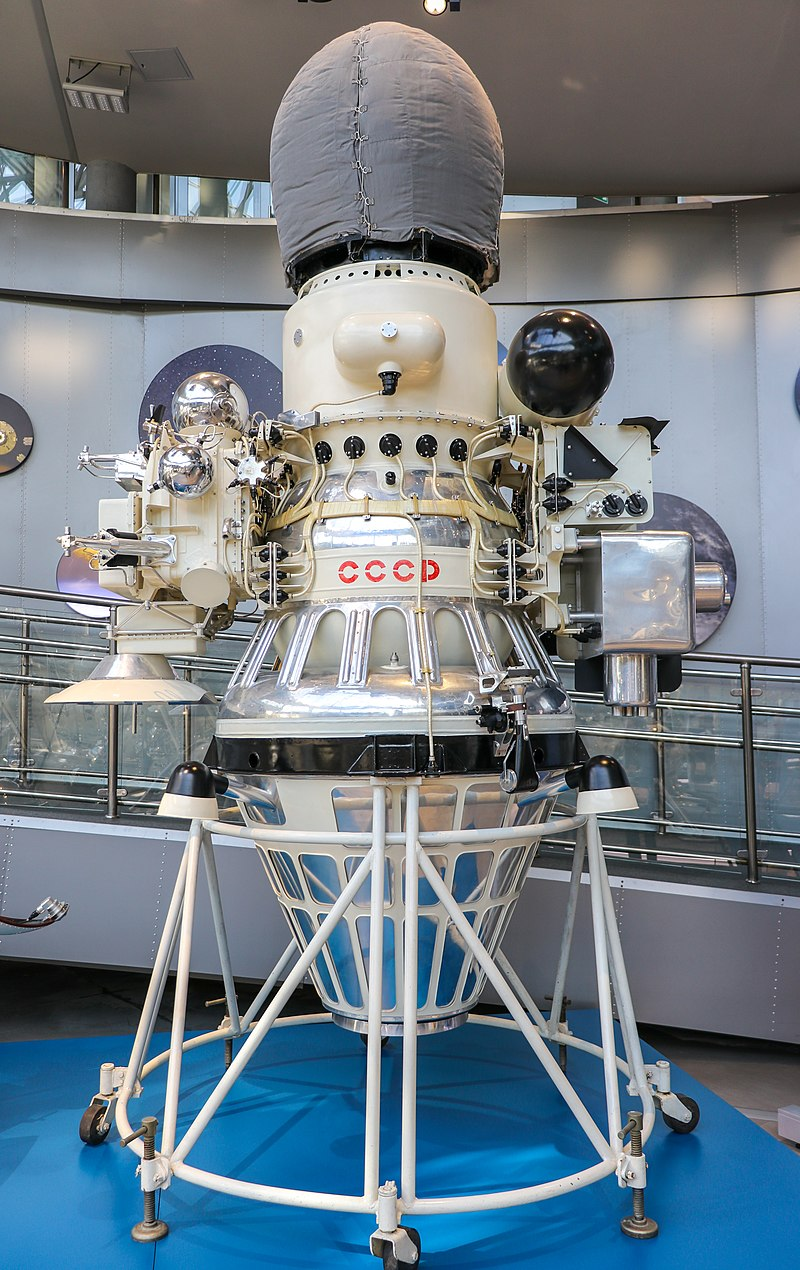
\includegraphics[width=0.3\textwidth]{Luna_9_Space_Probe}
	\caption{Модель межпланетной станции в Музее истории космонавтики имени К. Э. Циолковского}
\end{wrapfigure}

\noindent «Луна-9» — советская автоматическая межпланетная станция для изучения Луны и космического пространства. 

\noindent До неё было совершено одиннадцать попыток мягкой посадки на Луну по программе создания автоматических лунных станций типа Е-6. Только три аппарата достигли поверхности Луны, но разбились: «Луна-5», «Луна-7» и «Луна-8».

\noindent При реализации проекта были решены такие задачи, как запуск космических аппаратов в дальний космос с промежуточной околоземной орбиты, использование автономной астроориентации, коррекция траектории полета на большом удалении от Земли, осуществление прецизионного прицеливания и мягкая посадка на небесное тело, лишенное атмосферы.

\noindent Основным научным прибором, который планировалось доставить на Луну, была панорамная телевизионная камера. Кроме того, на борту станции находились приборы для регистрации космического излучения.

\noindent Ракета-носитель 8К78М («Молния») с аппаратом Е-6М стартовала 31 января 1966 года. Cтанция с разгонным блоком вышла на опорную орбиту, а затем вывела автоматическую станцию на заданную траекторию.
\begin{SCfigure}
	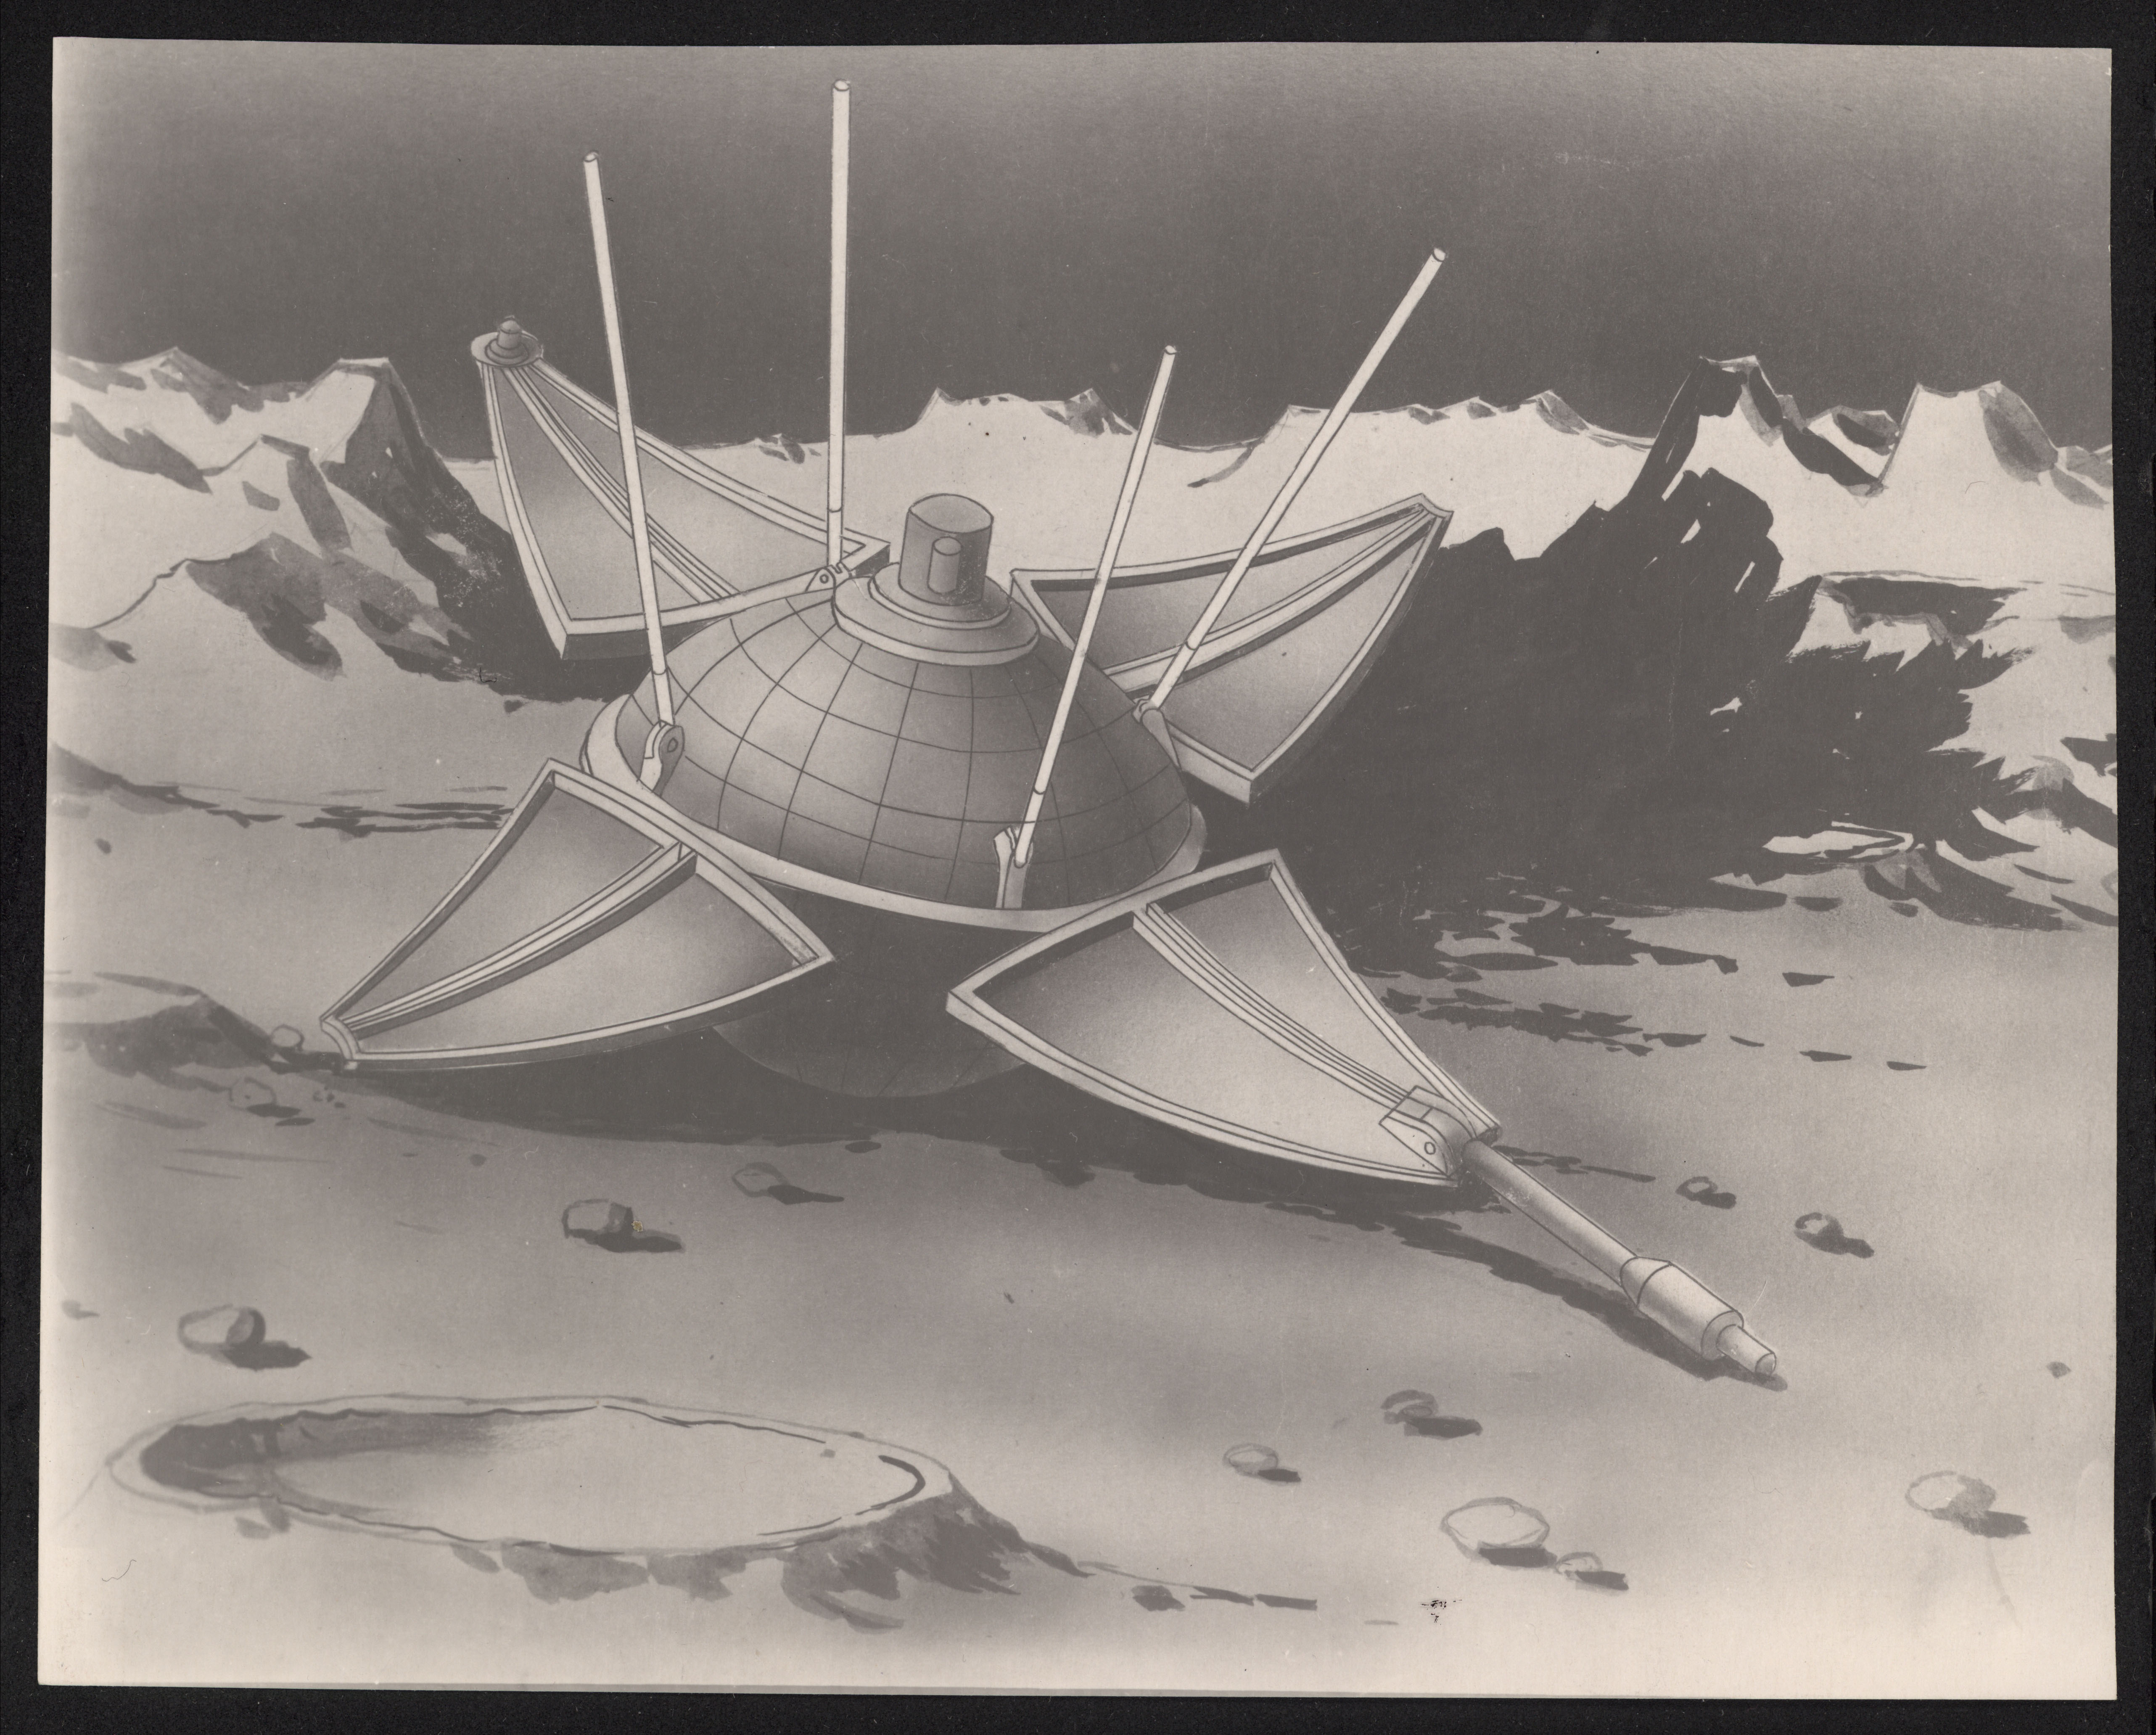
\includegraphics[width=0.5\textwidth]{4164397702}
	\caption{Плакат с художественным изображением автоматической лунной станции, иллюстривовавший первую пресс-конференцию по мягкой посадке <<Луна-9>>}
\end{SCfigure}
\noindent Подготовка к посадке началась 3 февраля 1966 года за пять часов до достижения цели. Перед торможением станция точно «поймала» лунную вертикаль, а затем, сбросив уже не нужные боковые отсеки, на высоте 75 км от лунной поверхности включила тормозной двигатель. И еще через несколько минут автоматическая лунная станция (АЛС), получившая официальное название, совершила мягкую посадку в точке с координатами 7°8‘ с.ш. и 64°22’ з.д. в районе океана Бурь, западнее кратеров Рейнер и Марий.
\subsection{Устройство станции}
\noindent Автоматическая станция состояла из двух частей: перелётного блока и автоматической лунной станции. Масса «Луны-9» 1538 кг при длине 2,7 метра.

\noindent Автоматическая лунная станция имела диаметр 58 см и массу 100 кг. Станция состояла из герметичного контейнера под давлением 1,2 атм. В контейнере устанавливались радиосистема, программно-временное устройство, аккумулятор, система терморегулирования и научные приборы. Четыре лепестковых антенны были расположены на верхней полусфере лунной станции и автоматически открывались после мягкой посадки, ориентируя её по вертикали. Два надувных баллона-амортизатора, закрывавшие станцию со всех сторон, смягчали прилунение. 
\section{Модели}
\subsection{Математическая модель}
\paragraph{Краткое описание} Составим уравнение изменение массы со временем, для описания того как изменяется скорость в каждый конкретный промежуток времени будем использовать уравнение Циолковского, для описания движения самого тела будем использовать второй закон Ньютона, также учитываем силу сопротивления воздуха.

\subsubsection{Необходимые уравнения}
\begin{itemize}
	\item Уравнение Циолковского (для нахождения модуля скорости в зависимости от массы): \[V = I_{sp} \times g_0 \times ln(\frac{M_f}{M_e}),\] где $I_{sp}$ - удельный импульс в $c$,  $M_f$ - полная масса ракеты с топливом, $M_e$ - пустая масса ракеты, $g$ - ускорение свободного падения.
	\item Закон всемирного тяготения: \[F = G\frac{m_1 m_2}{r^2},\] где $G$ - гравитационная постоянная, $m_1, m_2$ - массы тел, $r$ - расстояние между центрами тел.
	\item Уравнение Мещерского (для нахождения модуля ускорения): \[\vec{a} = \frac{\vec{F_p} + \vec{F}}{m_p},\] где $\vec{F}$ - внешние силы, действующие на тело (силы сопротивления воздуха), $\vec{F_p}$ - реактивная сила, обусловленная изменением массы движущегося тела, $m_p$ - масса тела.
	\item Формула коэффициента изменения массы: \[k = \frac{M_0 - M}{T},\] где $M_0$ - начальная масса ракеты, $M$ - масса ракеты после выработки топлива, $T$ - время работы двигателей.
	\item Уравнение расхода массы: \[m(t) = M-0 - kt.\]
	\item Расчет силы сопротивления воздуху при нахождении ракеты в атмосфере по упрощенной формуле лобового сопротивления: \[F = C_F \frac{\rho v^2}{2}S,\] где $\rho$ - плотность, зависящая от высоты, $v^2$ - квадрат вектора скорости, $S$ - харатерная площадь движущегося тела, $C_F$ - коэффициент формы.
	\item Расчет момента силы сопротивления, препятствующего изменению угловой скорости ракеты: \[M_{resist} = k \omega^2 \rho \frac{L}{2}.\]
\end{itemize}

\subsection{Физическая модель}

\begin{itemize}
	\item 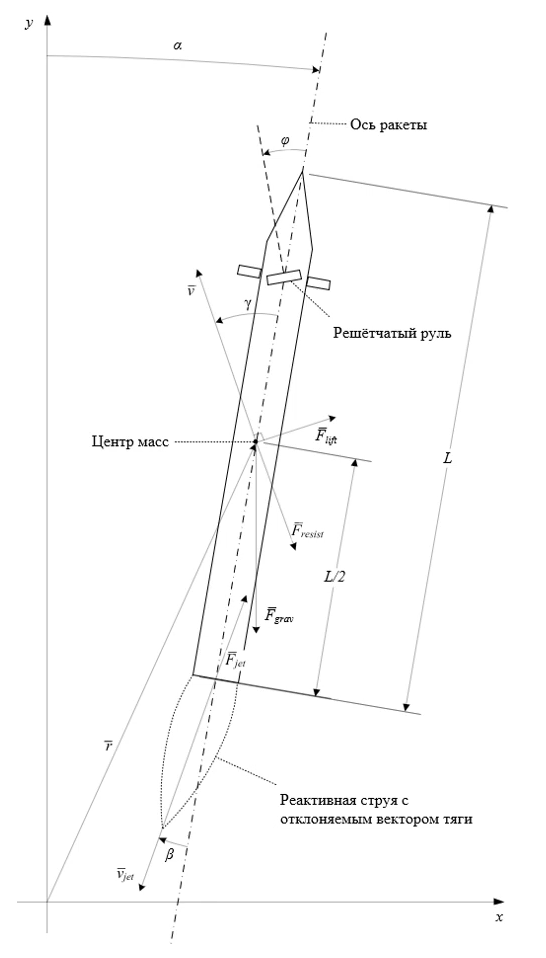
\includegraphics[width=0.3\textwidth]{rocket_scheme}	
	\item ракета рассматривается как стержень с равномерно распределенной плотностью, не смещенным центром массы;
	\item двумерная модель (движение в плоскости XY);
	\item учитывается поступательное и вращательное движение твердого тела;
	\item не учитывается кривизна Земли;
	\item атмосфера - идеальный газ с молярной массой 0,029 кг/моль, с температурой $T = 300 K$, плотность воздуха на высоте 0 м составляет 1 кг/$\mbox{м}^3$;
	\item постоянное гравитационное поле 9,8 м/$\mbox{с}^3$.
\end{itemize}

\section{Программная реализация}
Для симуляции, получения различного рода данных из kRPC напрямую в режиме реального времени существуют, например, язык kOS или модули для различных других языков программирования kRPC.

Мы используем kRPC из-за сложного поиска ошибок, дебаггинга на kOS и меньшей сложности написания кода.

Мы будем пользоваться (и ссылаться на документацию) модулем kRPC для языка программирования Python из-за динамической типизации и удобства написания кода относительно других доступных языков программирования (Lua, C-подобные, Java).

\begin{wrapfigure}{r}{0.3\textwidth} %this figure will be at the right
	\centering
	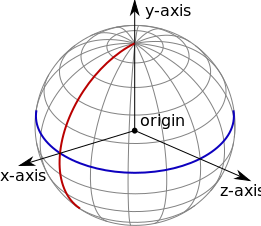
\includegraphics[width=0.3\textwidth]{celestial-body}
\end{wrapfigure}
Для реализации неподвижной сферической системы координат воспользуемся модулем \textit{non\tus rotating\tus reference\tus frame} из класса \textit{CelestialBody}. Точка начала отсчета находится на пересечении нулевого меридиана и Экватора. Координаты корабля в данный момент времени можно найти с помощью метода \textit{position(*система координат*)} класса \textit{Vessel}. Таким образом, можно найти различные тригонометрические значения угла.

...
\section{Симуляция}
Чтобы наша программа могла взаимодействовать с KSP, мы загрузили специализированный мод kRPC. Чтобы установить модификацию мы скачали файлы из интернета, после чего перенесли их в файлы KSP. Далее установили соединение через локальный сервер. Теперь с помощью функций данного мода мы можем получать данные о полете в любой момент времени и даже дистанционно управлять кораблем.

...

\section{Медиа}

\section*{Заключение}

\section*{Источники}
\begin{enumerate}
	\item \href{https://ru.wikipedia.org/wiki/%D0%9B%D1%83%D0%BD%D0%B0-9}{Луна-9 - Википедия: для описания миссии и исторической справки}
	\item \href{https://www.roscosmos.ru/29868/#1}{<<Есть мягкая посадка на Луну!>> - статья на странице Роскосмоса}
	\item \href{https://sites.google.com/view/kspmath/home}{The Kerbal Math and Physics Lab}
	\item \href{https://kerbalx.com/}{KerbalX - библиотека воздушных судов в KSP}
	\item \href{https://www.youtube.com/playlist?list=PLP3ZxgNn8T5IycT_nu3IgpLHhYrONjzsp}{Плейлист Лаборатории прикладных технологий ФАКТ МФТИ}
	\item \href{https://krpc.github.io/krpc/python/client.html}{Документация kRPC для языка Python}
	\href{https://forum.kerbalspaceprogram.com/index.php?/topic/130742-15x-to-122-krpc-control-the-game-using-c-c-java-lua-python-ruby-haskell-c-arduino-v048-28th-october-2018/}{Пост на Kerbal Space Program Forum о плагине для запуска сервера}
\end{enumerate}

\end{document}